\documentclass[a4paper,12pt, oneside]{book}

% \usepackage{fullpage}
\usepackage[italian]{babel}
\usepackage[utf8]{inputenc}
\usepackage{amssymb}
\usepackage{amsthm}
\usepackage{graphics}
\usepackage{amsfonts}
\usepackage{listings}
\usepackage{amsmath}
\usepackage{amstext}
\usepackage{engrec}
\usepackage{rotating}
\usepackage[safe,extra]{tipa}
%\usepackage{showkeys}
\usepackage{multirow}
\usepackage{hyperref}
\usepackage{mathtools}
\usepackage{microtype}
\usepackage{enumerate}
\usepackage{braket}
\usepackage{marginnote}
\usepackage{ulem}
\usepackage{pgfplots}
\usepackage{cancel}
\usepackage{polynom}
\usepackage{booktabs}
\usepackage{enumitem}
\usepackage{framed}
\usepackage{algorithm}
\usepackage{algpseudocode}
\usepackage{pdfpages}
\usepackage{pgfplots}
\usepackage[cache=false]{minted}

\usepackage[usenames,dvipsnames]{pstricks}
\usepackage{epsfig}
\usepackage{pst-grad} % For gradients
\usepackage{pst-plot} % For axes
\usepackage[space]{grffile} % For spaces in paths
\usepackage{etoolbox} % For spaces in paths
\makeatletter % For spaces in paths
\patchcmd\Gread@eps{\@inputcheck#1 }{\@inputcheck"#1"\relax}{}{}
\makeatother

\usepackage{tikz}\usetikzlibrary{er}\tikzset{multi
  attribute /.style={attribute ,double  distance =1.5pt}}\tikzset{derived
  attribute /.style={attribute ,dashed}}\tikzset{total /.style={double
    distance =1.5pt}}\tikzset{every  entity /.style={draw=orange ,
    fill=orange!20}}\tikzset{every  attribute /.style={draw=MediumPurple1,
    fill=MediumPurple1!20}}\tikzset{every
  relationship /.style={draw=Chartreuse2, fill=Chartreuse2!20}}
\newcommand{\key}[1]{\underline{#1}}

\usepackage{fancyhdr}
\pagestyle{fancy}
\fancyhead[LE,RO]{\slshape \rightmark}
\fancyhead[LO,RE]{\slshape \leftmark}
\fancyfoot[C]{\thepage}
\usepackage{tikz}
\usetikzlibrary{automata,positioning}


\title{Assignment 1, Bioinformatica}
\author{Davide Cozzi, 829827}
\date{}

\pgfplotsset{compat=1.13}
\begin{document}
\maketitle

\definecolor{shadecolor}{gray}{0.80}
\setlist{leftmargin = 2cm}
\newtheorem{teorema}{Teorema}
\newtheorem{definizione}{Definizione}
\newtheorem{esempio}{Esempio}
\newtheorem{corollario}{Corollario}
\newtheorem{lemma}{Lemma}
\newtheorem{osservazione}{Osservazione}
\newtheorem{nota}{Nota}
\newtheorem{esercizio}{Esercizio}

\renewcommand{\chaptermark}[1]{%
  \markboth{\chaptername
    \ \thechapter.\ #1}{}}
\renewcommand{\sectionmark}[1]{\markright{\thesection.\ #1}}
\tableofcontents
\chapter{esercizio 1}
\section{Versione 1}
Si assumano stringhe su $\Sigma=\{a,c,g,t,A,C,G,T\}$ indicizzate a partire dalla
posizione 0, per comodità.\\
L'algoritmo si divide in due parti:
\begin{enumerate}
  \item divisione in ``token'' delle due stringhe. A partire da ogni stringa si
  ottiene un vettore di sottostringhe di uguali caratteri
  \item confronto dei due vettori di sottostringhe
\end{enumerate}
%Assumendo in input le due stringhe $v$ e $w$, rispettivamente di lunghezza $n$ e
%$m$
%, si ha che la costruzione dei due vettori ha costo rispettivamente
%$\mathcal{O}(n)$ e $\mathcal{O}(m)$ mentre
%il confronto, possibile solo se i due vettori prodotti hanno lunghezza uguale
%$l$, è in $\mathcal{O}(l)$. \\
Si procede specificando che:
\begin{itemize}
  \item $length(X)$ restituisce la lunghezza di $X$, che sia una stringa o un
  vettore 
  \item $push(X,Y)$ effettua l'operazione di \texttt{push} di $Y$ nel
  vettore/stringa $X$
  \item $string(Y)$ effettua il cast di $Y$ a \texttt{string}
  \item $Y[i,e]$ specifica la sottostringa di $Y$ che va dall'indice $i$ incluso
  all'indice $e$ incluso
  \item $lowercase(Y)$ porta $Y$ in \textit{lowercase}
\end{itemize}
Si ha quindi la prima parte dell'algoritmo, che effettua la divisione in
``token''.
\newpage
\begin{esempio}
  Vediamo un esempio di input e output della funzione \texttt{Splitter}.
  \begin{itemize}
    \item \textbf{input}: \textit{"aaataaaggggccccctttttttttttttttcc"}
    \item \textbf{output}: \textit{["aaa", "t", "aaa", "gggg", "ccccc",
      "ttttttttttttttt", "cc"]} 
  \end{itemize}
\end{esempio}
Si ha quindi lo pseudocodice:
\begin{algorithm}[H]
  \begin{algorithmic}
    \Function{Splitter}{$s$}
    \State $result \gets \left[\,\,\,\right]$
    \State $n\gets length(s)$
    \State $last\_mismatch \gets 0$
    \If {$n==1$}
    \State $push(result, string(s[0]))$
    \State \textbf{return} $result$
    \EndIf
    \State $tmp \gets ""$
    \For {$i\gets 0$ \textbf{to} $n$}
    \If {$i > 0$ \textbf{and} $s[i-1]\neq s[i]$}
    %\State $tmp \gets s[last\_mismatch, i-1]$
    \State $push(result, tmp)$
    \State $tmp \gets ""$
    %\State $last\_mismatch \gets i$
    \EndIf
    \State $push(tmp, s[i])$
    \If {$i == (n-1)$}
    % \State $tmp \gets s[last\_mismatch, n-1]$
    % \State $push(result, tmp)$
    \State $push(result, tmp)$
    \EndIf
    \EndFor
    \State \textbf{return} $result$
    \EndFunction
  \end{algorithmic}
  \caption{Algoritmo per lo split in ``token'' delle stringhe}
\end{algorithm}
Una volta ottenuto il vettore dei ``token'' delle due sequenze in input basta
confrontare i due vettori.\\
Prima di vedere il confronto si specifica che:
\begin{itemize}
  \item le due sequenze vengono trasformate in \textit{lowercase} per praticità
  \item si assume che le due sequenze non possono essere stringhe vuote
  $\varepsilon$ 
\end{itemize}
Fatte queste assunzioni si può fare ancora un ultima osservazione prima di
procedere con l'algoritmo. Qualora i due vettori prodotti dalla funzione
\texttt{Splitter} fossero di lunghezza diversa allora l'algoritmo non potrà in
nessun caso dire che ci sia stata un'''infezione'' in quanto si assume che non
ci siano né \textit{gaps} né \textit{inserimenti}. In altri termini qualora i
due vettori siano di diversa cardinalità sicuramente, con queste premesse, non è
avvenuta alcuna infezione. Vediamo ora le altre casistiche. Si itera
contemporaneamente sull'elemento i-esimo dei due vettori e:
\begin{itemize}
  \item se i due elementi i-esimi presentano il primo carattere diverso allora,
  date le premesse, si specifica che non può essere avvenuta un'infezione
  \item se i due elementi i-esimi presentano il primo carattere uguale allora si
  procede confrontando i due elementi i-esimi (si assuma $X$ vettore relativo
  alla ``sequenza originale'' e $Y$ vettore relativo alla sequenze che si vuole
  dimostrare l'eventuale infezione):
  \begin{itemize}
    \item se il primo carattere è ``a'' allora la lunghezza di $Y[i]$ deve
    essere minore o uguale a 5 volte quella di $X[i]$, in quanto per ogni ``a''
    in $X[i]$ posso avere al più 5 ``a'' in $Y[i]$
    \item se il primo carattere è ``t'' allora la lunghezza di $Y[i]$ deve
    essere minore o uguale a 10 volte quella di $X[i]$, in quanto per ogni ``t''
    in $X[i]$ posso avere al più 10 ``t'' in $Y[i]$
    \item se il primo carattere è ``c'' o ``g'' allora la lunghezza di $Y[i]$
    deve essere maggiore o uguale di quella di $X[i]$, in quanto per ogni ``c''
    o ``g'' in  in $X[i]$ posso avere un numero indefinito di ``c'' o ``g'' in
    $Y[i]$ 
  \end{itemize}
\end{itemize}
\newpage
Si ha quindi il seguente pseudocodice dell'algoritmo, che ritorna $\top$ o
$\bot$ a seconda che sia possibile che $seq2$ sia una versione infettata di
$seq1$:
\begin{algorithm}[H]
  \begin{algorithmic}
    \Function{CheckInfection}{$seq1,seq2$}
    \If{$length(seq1) == 0$ \textbf{or} $length(seq2)==0$}
    \State \textbf{return} $\bot$
    \EndIf
    \State $vecseq1\gets Splitter(lowercase(seq1))$
    \State $vecseq2\gets Splitter(lowercase(seq2))$
    \State $check \gets \top$
    \If {$length(vecseq1)\neq length(vecseq2)$}
    \State \textbf{return} $\bot$
    \EndIf
    \State $j \gets length(vecseq1)$
    \For {$i\gets 0$ \textbf{to} $j$}
    \If {$vseq1[i][0] \neq vseq2[i][0]$ \textbf{or} $\neg check$}
    \State \textbf{return} $\bot$
    \EndIf
    \If {$vecseq1[i][0]==\,'a'$}
    \State $check \gets (length(vecseq2[i]) \leq 5\cdot length(vecseq1[i]))$
    \ElsIf {$vecseq1[i][0]==\,'t'$}
    \State $check \gets (length(vecseq2[i]) \leq 10\cdot length(vecseq1[i]))$
    \Else
    \State $check \gets (length(vecseq2[i]) \geq length(vecseq1[i]))$
    \EndIf
    \EndFor
    \State \textbf{return} $check$
    \EndFunction
  \end{algorithmic}
  \caption{algoritmo di verifica dell'infezione}
\end{algorithm}
\begin{esempio}
  Qualche esempio:
  \begin{itemize}
    \item \textbf{input}: "ATAGCTC" e \\"AAATAAAGGGGCCCCCTTTTTTTCC" 
    \item \textbf{output}: $\top$
  \end{itemize}
  infatti (si usano i colori per rappresentare i vari ``token'' dei vettori):
  \begin{center}
    \color{blue}A\color{green}T\color{blue}A\color{red}G\color{yellow}C\color{green}T\color{yellow}C\\ 
    \color{blue}AAA\color{green}T\color{blue}AAA\color{red}GGGG\color{yellow}CCCCC\color{green}TTTTTTT\color{yellow}CC
  \end{center}
  Avendo che tutti i vincoli sono rispettati.
  \newpage
  D'altro canto vediamo un esempio in cui non si può dire di avere una
  mutazione: 
  \begin{itemize}
    \item \textbf{input}: "ATAGCTC" e \\"AAATAAAAAAGGGGCCCCCTTTTTTTCC" 
    \item \textbf{output}: $\bot$
  \end{itemize}
  infatti (si usano i colori per rappresentare i vari ``token'' dei vettori):
  \begin{center}
    \color{blue}A\color{green}T\color{blue}A\color{red}G\color{yellow}C\color{green}T\color{yellow}C\\ 
    \color{blue}AAA\color{green}T\color{blue}AAAAAA\color{red}GGGG\color{yellow}CCCCC\color{green}TTTTTTT\color{yellow}CC
  \end{center}
  Avendo che il terzo ``token'' della prima stringa è {\color{blue}A} mentre
  quello della seconda stringa è {\color{blue}AAAAAA}, avendo che viene rotto il
  vincolo per il quale per ogni $A$ posso avere al più 5 $A$ nella mutazione.\\
  Un altro esempio in cui non si può dire di avere una
  mutazione è: 
  \begin{itemize}
    \item \textbf{input}: "ATAGCTC" e \\"AAACCTAAAAAAGGGGCCCCCTTTTTTT" 
    \item \textbf{output}: $\bot$
  \end{itemize}
   infatti (si usano i colori per rappresentare i vari ``token'' dei vettori):
  \begin{center}
    \color{blue}A\color{green}T\color{blue}A\color{red}G\color{yellow}C\color{green}T\color{yellow}C\\ 
    \color{blue}AAA\color{yellow}CC\color{green}T\color{blue}AAAAAA\color{red}GGGG\color{yellow}CCCCC\color{green}TTTTTTT
  \end{center}
  In quanto i due secondi ``token'', {\color{green}T} e {\color{yellow}CC},
  corrispondono a caratteri diversi.
\end{esempio}
\newpage
\section{Versione 2}
Si assumano stringhe su $\Sigma=\{a,c,g,t,A,C,G,T\}$ indicizzate a partire dalla
posizione 0, per comodità.\\
Indico anche una versione intuitivamente più semplice. In questo caso si scorre
la sequenze che si suppone essere 
originale, tenendo conto dei caratteri uguali ripetuti. Appena si ha un cambio
di carattere si verifica se nella sequenza che si vuole dimostrare essere una
mutazione di quella originale si ha una corretta sequenza di caratteri secondo
la specifica.\\
Si ha che:
\begin{itemize}
  \item per comodità le sequenze sono riportate in lowercase e si assume che, in
  presenza di anche solo una sequenza nulla, l'algoritmo restituisce $\bot$
  \item \texttt{seq1} e \texttt{seq2} sono rispettivamente la sequenza originale
  al sequenza che si vuole dimostrare essere la mutazione
  \item \texttt{co} e \texttt{cm} sono le variabili che ogni volta
  accumulano il conteggio dei caratteri uguali consecutivi rispettivamente sulla
  sequenza originale e su quella che si suppone mutata
  \item $i$ e $j$ sono rispettivamente gli indici per la prima e per la seconda
  sequenza 
\end{itemize}
In poche parole si itera sulla sequenza originale, aggiornando di volta in volta
il contatore relativo finché si ha lo stesso carattere. Nel momento in cui si ha
un cambiamento o si è arrivato all'ultimo carattere della sequenza si ferma il
conteggio e si verifica il conteggio sulla seconda sequenza (anche in questo
caso facendo attenzione a non andare \textit{out of bounds}). Qualora la seconda
sequenza presenti, all'indice a cui si è arrivati con l'algoritmo, un carattere
diverso da quello della prima si può restituire $\bot$. Controllando la
seconda sequenza si aggiorna il rispettivo contatore e l'indice. Una volta che
anche sulla seconda sequenza si ha un cambio di carattere o si è arrivati alla
fine si confrontano i due contatori secondo le specifiche (ad esempio se nella
stringa originale avevo due ``a'' consecutive ne posso avere al più 10 in quella
che si vuole verificare essere la mutazione). Finito questo controllo si
azzerano i contatori e si verifica che, qualora la sequenza originale sia stata
visitata interamente, anche la seconda sia conclusa. In caso contrario si
restituisce $\bot$.\\
Si ha quindi il seguente pseudocodice.
\begin{algorithm}[H]
  \begin{algorithmic}
    \Function{CheckInfection}{$seq1,seq2$}
    \State $m \gets length(seq1)$
    \State $n \gets length(seq2)$
    \If{$m == 0$ \textbf{or} $n==0$}
    \State \textbf{return} $\bot$
    \EndIf
    \State $seq1\gets lowercase(seq1)$
    \State $seq2\gets lowercase(seq2)$
    \State $co \gets 0$
    \State $cm \gets 0$
    \State $j \gets 0$
    \For {$i\gets 0$ \textbf{to} $m$}
    \State $co \gets co+1$
    \If {$i==n-1$ \textbf{or} $seq1[i]\neq seq[i+1$}
    \If {$seq1[i]\neq seq2[j]$}
    \State \textbf{return} $\bot$
    \EndIf
    \While {$j \neq n-1$ \textbf{and} $seq2[j]==seq2[j+1]$}
    \State $cm \gets cm+1$
    \State $j \gets j+1$
    \EndWhile
    \State $cm \gets cm+1$
    \State $j \gets j+1$
    \If {$seq1[i]==\,'a'$ \textbf{and} $cm \leq 5\cdot co$}
    \State $check \gets \top$
    \ElsIf {$seq1[i]==\,'t'$ \textbf{and} $cm \leq 10\cdot co$}
    \State $check \gets \top$
    \ElsIf {($seq1[i]==\,'c'$ \textbf{or} $seq1[i]==\,'g'$) \textbf{and}
    $cm \geq co$} 
    \State $check \gets \top$
    \Else
    \State  \textbf{return} $\bot$
    \EndIf
    \State $co \gets 0$
    \State $cm \gets 0$
    \If {$i==m-1$ \textbf{and} $j\neq n$}
    \State  \textbf{return} $\bot$
    \EndIf
    \EndIf
    \EndFor
    \State \textbf{return} $check$
    \EndFunction
  \end{algorithmic}
  \caption{algoritmo di verifica dell'infezione, seconda versione}
\end{algorithm}
Dal punto di vista pratico questo secondo algoritmo evita la fase di
preprocessing vista nel primo algoritmo con la funzione
\texttt{Splitter}. Anziché avere a priori le sottostringhe di cui confrontare le
lunghezze tiene conto di volta in volta dei caratteri uguali consecutivi,
confrontando i contatori (motivo per cui anche gli esempi possono essere
riadattati anche a questa seconda versione). Dal
punto di vista computazionale, assumendo che la funzione \texttt{length} abbia
costo lineare si ha in entrambi i casi un tempo quadratico nel caso peggiore,
anche se si potrebbe fare uno studio più approfondito. 
\chapter{Esercizio 2}
Si assumano stringhe su $\Sigma=\{a,c,g,t,A,C,G,T\}$ (anche se come
nell'esercizio precedente poi si procederà con il \texttt{lowercase})
indicizzate a partire dalla posizione 0, per comodità.\\
Si fanno le seguenti assunzioni:
\begin{itemize}
  \item si assume che le mutazione siano solo cambi di base, non avendo quindi
  inserzioni o delezioni
  \item si assume che, non avendo inserzioni o delezioni, le due sequenze siano
  di egual lunghezza per poter avere un input valido per l'algoritmo
  \item si assume che si può avere una mutazione solo dopo almeno 5 basi non
  mutate 
  \item si assume che la prima base della sequenza può mutare
  \item si assume che le sequenze siano tali per cui il loro \textit{kmer-set}
  coincida con il loro \textit{spettro}. In altri termini le sequenze sono tali
  per cui si hanno solo \textit{kmer} univoci
\end{itemize}
In base alle assunzioni precedenti si può anche assumere che, calcolati i due
\textit{spettri}, che sono \textit{spettri senza ripetizioni}, relativi alle due
sequenze, si abbia che essi siano di cardinalità uguale. Per verificare che il
\textit{kmer-set} sia della stessa cardinalità dello spettro basta verificare
che, assumendo $kmers$ il \textit{kmer-set} (calcolato per un certo $k$) di una
certa sequenza $seq$, non valga: 
\[length(kmers) \neq length(seq)-(k-1)\]
Procediamo quindi descrivendo l'idea dietro l'algoritmo. L'idea principale è
quella di calcolare i \textit{kmer} di una lunghezza $k$ non causale e di
evitare confronti inutili. Assumendo di avere che una mutazione è possibile sse
almeno le 5 basi precedenti non sono mutazioni, in quanto dopo una mutazione
abbiamo assunto esserci almeno 5 basi non mutate, sono di fronte ad un caso
``limite'' del tipo:
\begin{center}
  \textit{{\color{red}M}BBBBB{\color{red}M}}
\end{center}
Indicando con $M$ le mutazioni e con $B$ le basi non mutate. Ne segue
immediatamente che \textit{kmer} calcolati con $k=6$ sono i \textit{kmer} di
cardinalità massima tali per cui posso avere al più una singola mutazione per
\textit{kmer}. \\
Indicando con $seq1$ la sequenza di riferimento e con $seq2$ la sequenza mutata
si ha quindi che, per le assunzioni fatte, posso fare un confronto ``1:1'' dei
\textit{kmer-set}, sapendo che essi sono di cardinalità uguale.\\
Si noti però che un confronto diretto sarebbe ``inutile'' in quanto, avendo
sicuramente almeno 5 basi non mutate dopo una mutazione posso saltare il
confronto di 5 \textit{kmer}, in quanto tutti e 5 aggiungerebbero in coda una
base sicuramente non mutata. Inoltre, per le assunzioni fatte, è possibile anche
solo confrontare, di volta in volta, i due simboli finali dei due \textit{kmer}
e non i \textit{kmer} interi in quanto tutto il prefisso del \textit{kmer}, che
termina in penultima posizione della stringa, è stato già verificato negli step
precedenti. Qualora il simbolo finale sia diverso si è di fronte ad una
mutazione e, avendo \textit{kmer-set} di uguale cardinalità e quindi
confrontando sempre i due \textit{kmer} i-esimi, è possibile risalire all'indice
della mutazione basandosi su tale $i$ e sulla lunghezza dei \textit{kmer},
quindi $6$.\\
Una volta individuata la mutazione si procede a salvare in una struttura
adeguata le seguenti informazioni:
\begin{itemize}
  \item base presente nella sequenza di riferimento, \texttt{b1}
  \item base mutata presente nella seconda sequenza, \texttt{b2}
  \item indice della mutazione, \texttt{i}
\end{itemize}
In merito si assume che \texttt{newMutation(b1, b2, i)} restituisca una
mutazione con le specifiche indicate come argomento.\\
Bisogna fare un'ultima osservazione. Si è assunto che la primissima base possa
subire mutazione. Si verifica quindi se le due basi iniziali siano diverse e,
qualora lo fossero, si aggiunge la mutazione e ci si sposta ai due \textit{kmer}
di posizione $1$ nei due \textit{kmer-set}, sapendo che essi non conterranno
sicuramente la prima base delle rispettive sequenze e quindi, per le assunzioni
fatte, continueranno a contenere al più una mutazione, nell'ultimo
carattere. Dopo questa osservazione 
si procede regolarmente con l'algoritmo.\\
Per praticità l'algoritmo restituisce una tupla contenente:
\begin{enumerate}
  \item il vettore delle mutazioni
  \item un booleano che segnala se i vincoli del problema sono stati tutti
  rispettati 
\end{enumerate}
Quindi si hanno vari casi:
\begin{itemize}
  \item un vettore di mutazioni non nullo (in tal caso sicuramente il booleano
  presenta $\top$)
  \item un vettore di mutazioni nullo e in tal caso:
  \begin{itemize}
    \item se il booleano è $\top$ significa che le due sequenze rispettano tutti
    i vincoli ma non si hanno mutazioni
    \item se il booleano è $\bot$ significa che qualche vincolo è stato
    infranto, ovvero stringhe di lunghezza diversa, stringhe nulle e stringhe
    che prevedono \textit{kmer} non univoci
  \end{itemize}
\end{itemize}
\textit{L'assunzione di avere distanza 5 tra ogni mutazione non viene verificata
  e viene assunta come assioma}.\\
Vediamo quindi prima lo pseudocodice e poi qualche esempio.\\
Esplicitiamo prima la funzione \texttt{getKmers} che, data una sequenza $seq$ e
un intero $k$, restituisce un vettore di stringhe, che per le assunzioni è sia
il \textit{kmer-set} che lo \textit{spettro}, mantenendo l'ordine, quindi il
\textit{kmer} che nel vettore ha indice i è il \textit{kmer} che inizia
all'indice $i$ della sequenza. Quest'ultimo ragionamento è possibile solo grazie
alle assunzioni fatte: \textit{kmer} non univoci non permetterebbero questo. Con
$s[i,j]$ si intende la sottostringa di $s$ dall'indice $i$ all'indice $j$
inclusi. Con $s[i,]$ si intende il suffisso di $s$ che inizia all'indice $i$.
\begin{algorithm}[H]
  \begin{algorithmic}
    \Function{getKmers}{$seq$, $k$}
    \State $kmers \gets [\,\,\,]$
    \While {$length(seq)\geq k$}
    \State $push(kmers, seq[0,k-1])$
    \State $seq gets seq[1,]$
    \EndWhile
    \State \textbf{return} $kmers$
    \EndFunction
  \end{algorithmic}
  \caption{Funzione di calcolo dei \textit{kmer}}
\end{algorithm}
\textit{Si noti che la funzione consuma la sequenza ma potrebbe essere
  facilmente editato l'algoritmo per evitare questa cosa}.
\newpage
Passiamo ora allo pseudocodice principale.
\begin{algorithm}[H]
  \small
  \begin{algorithmic}
    \Function{CheckMutation}{$seq1$, $seq2$}
    \If{$length(seq1)\neq length(seq2)$}
    \State \textbf{return} $([\,\,\,],\bot)$
    \EndIf
    \If{$length(seq1)==0$ \textbf{or} $length(seq2)==0$}
    \State \textbf{return} $([\,\,\,],\bot)$
    \EndIf
    \State $muts \gets [\,\,\,]$
    \State $i\gets 0$
    \State $n\gets length(seq1)$
    \State $seq1\gets lowercase(seq1)$
    \State $seq2\gets lowercase(seq2)$
    \If{$seq1[0]\neq seq2[0]$}
    \State $push(muts, newMutation(seq1[0], seq2[0], 0))$
    \State $i \gets index+1$
    \EndIf
    \State $kmers1\gets getKmers(seq1,6)$
    \State $kmers2\gets getKmers(seq2,6)$
    \If{$length(kmers1)\neq n-(k-1)$ \textbf{or} $length(kmers2)\neq n-(k-1)$}
    \State \textbf{return} $([\,\,\,],\bot)$
    \EndIf
    \While {$i < length(kmers1)$}
    \If{$kmers1[i][5]\neq kmers2[i][5]$}
    \State $push(muts, newMutation(kmers1[i][5], kmers2[i][5], (k-1)+i))$
    \State $i\gets i+k$
    \Else
    \State $i\gets i+1$
    \EndIf
    \EndWhile
    \State \textbf{return} $(muts, \top)$
    \EndFunction
  \end{algorithmic}
  \caption{}
\end{algorithm}
Dove con $i$ teniamo traccia dei \textit{kmer} da confrontare, eventualmente
saltando i confronti superflui sopra descritti.
\newpage
Vediamo quindi qualche esempio.
\begin{esempio}
  Siano date in input:
  \begin{itemize}
    \item atcttgcattaccgccccaatc
    \item atcttacattaccgtcccaacc
  \end{itemize}
  Le due sequenze rispettano tutte le assunzioni.\\
  Calcolati i \textit{kmer} si procede con il confronto, sapendo che le due
  sequenze iniziano con la stessa base. L'indice dell'enumerazione corrisponde
  all'indice $i$ dell'algoritmo.
  \begin{enumerate}[start=0]
    \item confronto "atcttg" con "atctta". Ho un mismatch tra gli ultimi simboli
    ``g'' e ``a'', che sono all'indice 5 essendo noi al \textit{kmer} di indice
    0 (si ha infatti $(6-1)+0=5$). Aggiungo quindi la mutazione \texttt{(g,a,5)}
    e aggiorno l'indice al valore $i+6$, ovvero, in questo caso, $6$. Salto
    quindi tutti i confronti e riparto dal 6
    \item \sout{confronto "tcttgc" con "tcttac"}
    \item \sout{confronto "cttgca" con "cttaca"}
    \item \sout{confronto "ttgcat" con "ttacat"}
    \item \sout{confronto "tgcatt" con "tacatt"}
    \item \sout{confronto "gcatta" con "acatta"}
    \item confronto "cattac" con "cattac". Non ho mismatch quindi faccio $i+1$ e
    basta andando al confronto successivo
    \item confronto "attacc" con "attacc". Non ho mismatch quindi faccio $i+1$ e
    basta andando al confronto successivo
    \item confronto "ttaccg" con "ttaccg". Non ho mismatch quindi faccio $i+1$ e
    basta andando al confronto successivo
    \item confronto "taccgc" con "taccgt". Ho un mismatch tra gli ultimi simboli
    ``c'' e ``t'', che sono all'indice 14 essendo noi al \textit{kmer} di indice
    9 (si ha infatti $(6-1)+9=14$). Aggiungo quindi la mutazione
    \texttt{(c,t,14)} 
    e aggiorno l'indice al valore $i+6$, ovvero, in questo caso, $15$. Salto
    quindi tutti i confronti e riparto dal 15
    \item \sout{confronto "accgcc" con "accgtc"}
    \item \sout{confronto "ccgccc" con "ccgtcc"}
    \item \sout{confronto "cgcccc" con "cgtccc"}
    \item \sout{confronto "gcccca" con "gtccca"}
    \item \sout{confronto "ccccaa" con "tcccaa"}
    \item confronto "cccaat" con "cccaac". Ho un mismatch tra gli ultimi simboli
    ``t'' e ``c'', che sono all'indice 20 essendo noi al \textit{kmer} di indice
    15 (si ha infatti $(6-1)+15=20$). Aggiungo quindi la mutazione
    \texttt{(t,c,20)} 
    e aggiorno l'indice al valore $i+6$, ovvero, in questo caso, $26$. Essendo
    l'indice maggiore stretto della cardinalità del \textit{kmer-set},
    interrompo l'esecuzione, sapendo che comunque non potrei avere in ogni caso
    ulteriori mutazioni
    \item \sout{confronto "ccaatc" con "ccaacc"}
  \end{enumerate}
\end{esempio}
\begin{esempio}
  Più brevemente vediamo un altro input:
  \begin{itemize}
    \item tatcttgcattaccgccccaatc
    \item gatcttacattaccgtcccaacc
  \end{itemize}
  In questo casi si noti come la prima base non combaci, si procede quindi
  salvando la mutazione \texttt{(t,g,0)} e facendo iniziare il confronto tra i
  \textit{kmer} di indice 1, ovvero ``atcttg'' e ``atctta'', proseguendo poi
  come nell'esempio precedente.
\end{esempio}
Per pura curiosità si può fare anche un piccolo ragionamento ulteriore. Con le
assunzioni date si può costruire un \textbf{grafo di De Brujin} delle due
stringhe e vedere che non si hanno cicli, non essendoci \textit{kmer} non
univoci all'interno di ciascuna stringa. Le mutazioni possono essere quindi
viste come le coppie di caratteri 
che etichettano l'inizio di una \textbf{bubble} nel grafo, ovvero le etichette
degli archi di un nodo che ha due archi uscenti, Vista l'essenza di
cicli, si ha che il primo \textit{kmer} calcolato per ciascuna delle due
sequenze (potrebbero essere due diversi) è un nodo privo di archi entranti,
essendo quindi un nodo \textit{source}, e
l'ultimo nodo calcolato per ciascuna delle due
sequenze (potrebbero essere due diversi) è un nodo privo di archi uscenti,
essendo un nodo \textit{sink}. È quindi possibile ragionare in modo analogo a
sopra, saltando il confronto tra i \textit{kmer} di nodi che formano i due rami
di una \textbf{bubble} e tenendo conto del numero di nodi per l'indice della
mutazione. \\
Qualora si abbia una mutazione nella prima base allora si avranno due
nodi privi di archi entranti che puntano però allo stesso nodo. Si procede
quindi aggiungendo la prima base come mutazione e proseguendo con il
ragionamento visto sopra a partire da questo nodo a cui puntano.\\
A seguire i due grafi relativi ai due esempi, dove è possibile verificare quanto
detto. Si noti che senza ulteriori assunzioni si perde esplicita referenza di
quale base che muta appartiene alla sequenza di riferimento o a quella mutata,
ma un controllo per capirlo è facilmente eseguibile usando l'indice.
\begin{figure}[H]
  \centering
  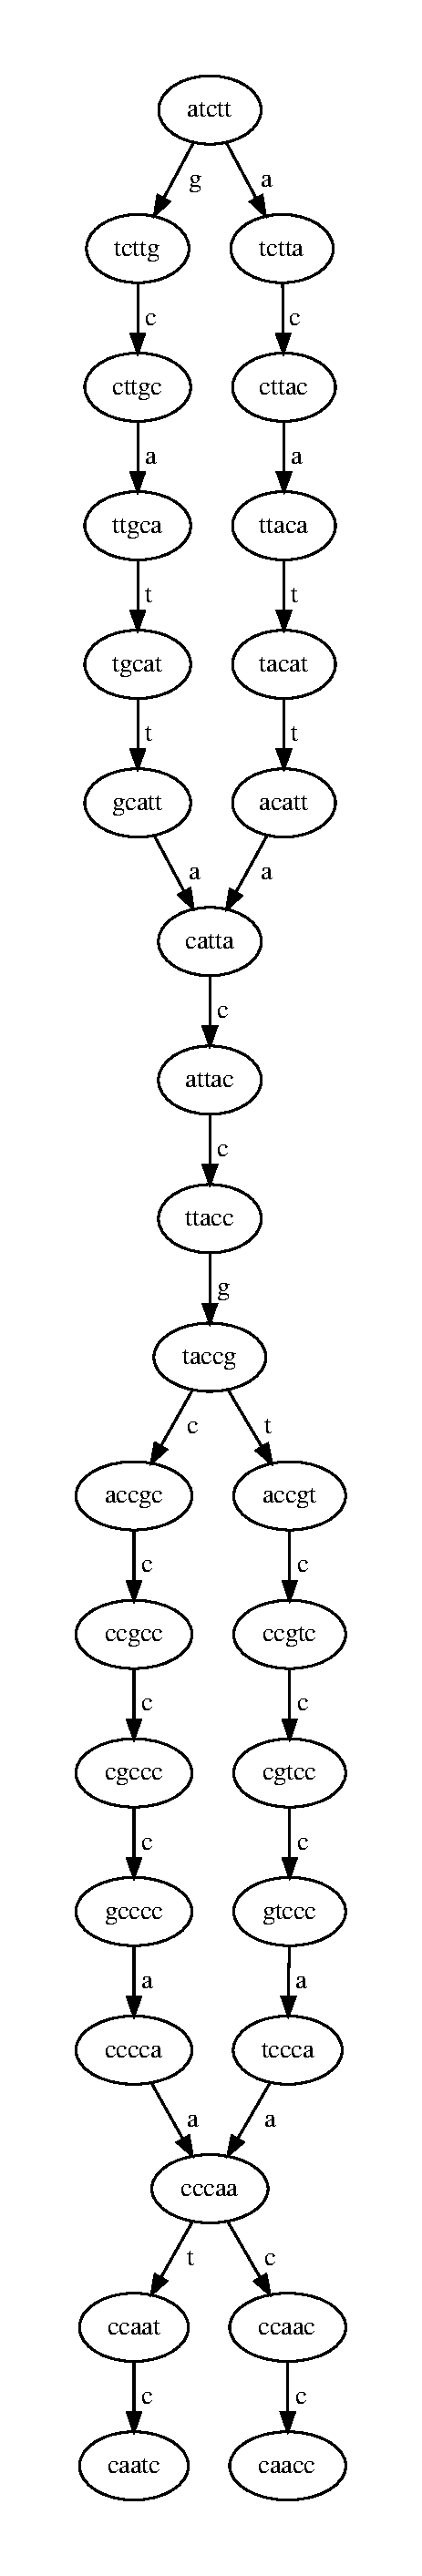
\includegraphics[scale = 0.33]{img/mut.pdf}
  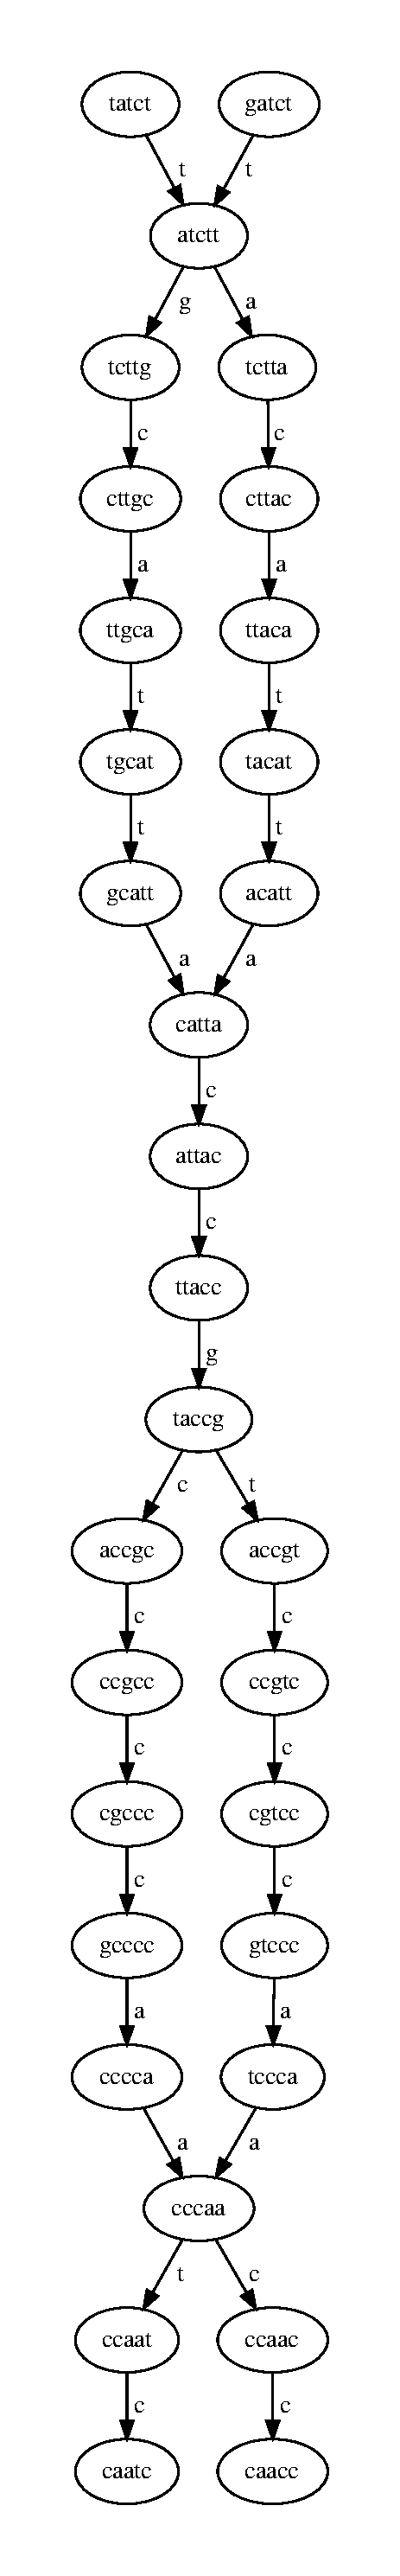
\includegraphics[scale = 0.33]{img/mutns.pdf}
\end{figure}
\chapter{Esercizio 3}
La \textbf{distanza di Hamming} tra due stringhe, che si assumono di uguale
lunghezza, è 
il numero di indici per i quali i due caratteri associati sulle due stringhe
sono diversi. È quindi un conteggio delle sostituzioni necessarie per passare da
una stringa all'altra.\\
Ipotizzando di voler studiare la distanza di Hamming tra due sequenze tramite la
griglia estesa si può ipotizzare di ragionare solo in termini di una delle due
sequenze, ovvero considerare i pesi degli archi in ottica di una sola delle due
sequenze, come in figura \ref{fig:pes3}. Si associano quindi i seguenti pesi:
\begin{itemize}
  \item $w(diagonale)=0$
  \item $w(verticale)=0$
  \item $w(orizzontale)=1$
\end{itemize}
o, in modo speculare se si vuole ragionare sull'altra sequenza:
\begin{itemize}
  \item $w(diagonale)=0$
  \item $w(verticale)=1$
  \item $w(orizzontale)=0$
\end{itemize}
\begin{figure}
  \centering
  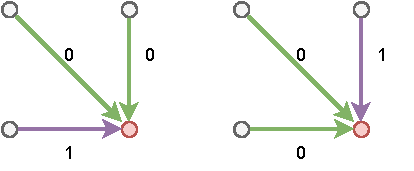
\includegraphics[scale = 1.3]{img/es31.pdf}
  \caption{Rappresentazione grafica dei pesi degli archi.}
  \label{fig:pes3}
\end{figure}
Dove, in entrambi i casi, gli archi diagonali rappresentano un match mentre, a
seconda, gli archi verticali o quelli orizzontali tengono conto dei mismatch.\\
A questo punto si cerca il cammino di peso minimo che parte dal nodo
\textit{source}, posto in alto a sinistra, e arriva al nodo \textit{sink}, posto
in basso a destra. Essendo il nodo sink in posizione $(n,n)$, assumendo le due 
sequenze lunghe $n$, garantisco che, calcolando il cammino che parte dal nodo
source $(0,0)$ e arriva in quel nodo, si abbia il valore della
distanza di Hamming, che prevede stringhe di ugual lunghezza. I vari valori
degli altri nodi sono da considerarsi ``temporanei'' e non rappresentanti una
distanza di Hamming. Potenzialmente però tutti e soli i nodi $(i,i)$, con
$i\in[1,n)$, oltre quindi al nodo sink, potrebbero essere i nodi di fine di
potenziali cammini dal source per calcolare la distanza di Hamming tra le
sottostringhe di lunghezza $i$ delle due stringhe in input.\\
Prendendo, ad esempio, in input:
\begin{itemize}
  \item AAAGTTC
  \item AAACTTT
\end{itemize}
Si ha un cammino minimo (non l'unico), assumendo costo degli archi in
orizzontale pari a 1 e in verticale pari a 0, del tipo:
\begin{figure}[H]
  \centering
  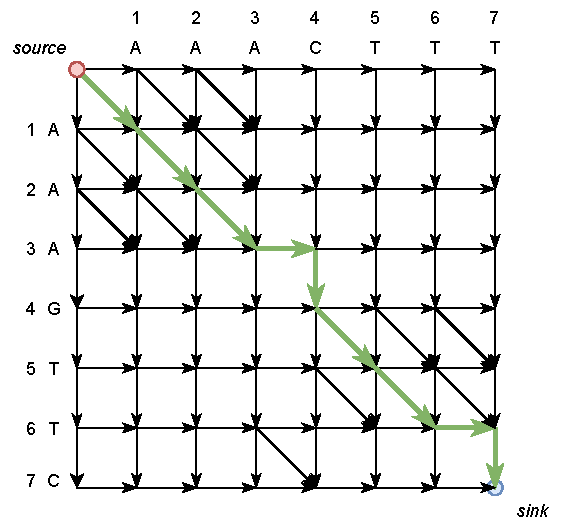
\includegraphics[scale = 1]{img/es3.pdf}
\end{figure}
\noindent
Dove in verde è segnato il cammino minimo scelto. Avendo solo due archi
orizzontali, che ricordiamo avere peso 1 mentre gli altri hanno peso nullo,
possiamo concludere che la distanza di Hamming tra le due stringhe è 
pari a 2.\\
Per il ragionamento fatto sopra, se mi fermassi in $(3,3)$, per $i=3$, avrei la
distanza di Hamming tra AAA e AAA. Il cammino dal source a $(3,3)$ è formato da
sole diagonali e quindi ha costo 0, che è appunto al distanza di Hamming tra le
due sottostringhe.
\chapter{Esercizio 4}
Il problema della \textbf{longest common substring} si pone l'obiettivo di
estrarre, a partire da due stringhe di lunghezza arbitraria, anche non uguale,
la sottostringa, comune ad entrambe, più lunga.\\
Dal punto di vista della griglia si assegnano i seguenti pesi (come da figura
\ref{fig:pes4}): 
\begin{itemize}
  \item $w(diagonale)=1$
  \item $w(verticale)=-i$
  \item $w(orizzontale)=-j$
\end{itemize}
\begin{figure}
  \centering
  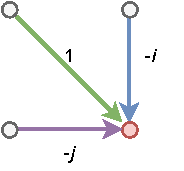
\includegraphics[scale = 1.3]{img/es41.pdf}
  \caption{Rappresentazione grafica dei pesi degli archi. Si ricorda che nel
    nodo finale, in rosso,
    posso comunque avere solo valori $\geq 0$}
  \label{fig:pes4}
\end{figure}
Dove gli archi diagonali rappresentano un match ed $i$ e $j$ sono gli indici che
scorrono le due stringhe, ovvero rispettivamente sulle righe e sulle colonne.\\
Si assume che i nodi abbiano valore $x\geq 0$ quindi
\textbf{qualora si ottenga un valore negativo come risultato dopo
  l'attraversamento dell'arco viene messo il valore 0}.\\
Quando si ha un match quindi il nodo finale ha valore pari a uno più il valore
del nodo sorgente dell'arco diagonale.\\
Si ragiona quindi tenendo traccia del valore massimo raggiungo, tenendo traccia,
per una maggior efficienza, anche delle coordinate. Una volta completata la
griglia si avrà che il valore massimo corrisponde al nodo \textit{sink} del
cammino composto dalla più lunga sequenza possibile di archi diagonali
consecutivi. Qualsiasi altra ``operazione'', con archi orizzontali o diagonali,
comporta infatti una perdita di punteggio e ogni volta che un cammino diagonale
termina viene azzerato il punteggio, tramite pesi negativi pesati sugli
indici. Azzerando ogni volta si permette di avere la costruzione di un eventuale
cammino diagonale che assegna man mano il valore corrispondente alla lunghezza
del cammino stesso, avendo che la diagonale pesa 1. Il valore massimo quindi
altro non è che  
la lunghezza della \textit{longest common substring}. Sapendo che archi
diagonali corrispondono a match tra le due sequenze si ottiene che tale cammino
corrisponde alla \textit{longest common substring}. \\
Volendo si può scegliere di salvare in un vettore i valori massimi qualora
coincidano, per ottenere eventuali più \textit{longest common substring} qualora
ce ne siano.\\
In altri termini si cerca il sottocammino più pesante.\\
ipotizzando di non ``azzerare'' ogni volta in caso di mismatch otterrei comunque
una griglia dover il nodo massimo mi permetterebbe di risalire la diagonale
ritrovando la \textit{longest common substring} ma tale nodo non potrebbe avere
come valore la lunghezza della stessa, in quanto non ricomincerei il conto da 0
ogni volta che creo un nuovo cammino fatto di diagonali.
Per ricostruire la \textit{longest common substring} si parte dal nodo
\textit{sink}, come detto definito dal valore massimo calcolato. Si aggiunge il
carattere corrispondente e si risale tutto il cammino diagonale, aggiungendo di
volta in volta in testa il carattere letto. Ci si ferma quindi quando non si ha
più un nodo il cui punteggio è stato ottenuto tramite un arco diagonale.

Vediamo quindi un esempio pratico. Siano date:
\begin{itemize}
  \item AAACGCGCTTTTTCCCAT
  \item AAAGGGGCGCGCTTTTTAAA
\end{itemize}
\newpage
Si costruisce quindi la griglia e si identifica il cammino diagonale più lungo:
\begin{figure}[H]
  \centering
  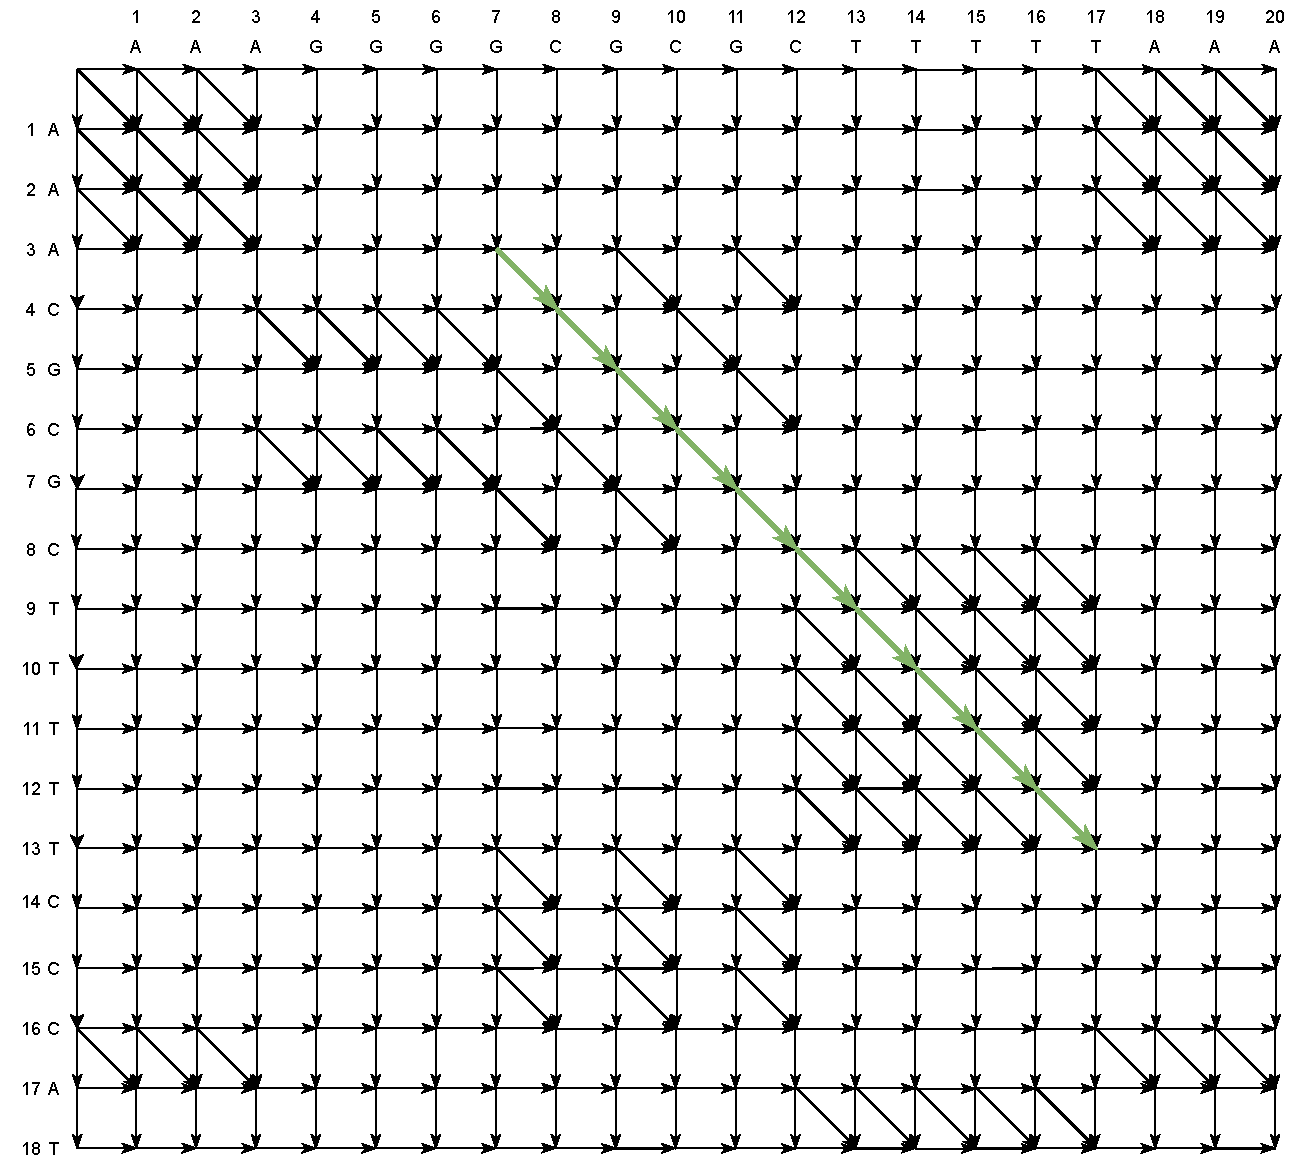
\includegraphics[scale = 0.62]{img/es4.pdf}
\end{figure}
Ricostruendo si ha che tale cammino identifica un massimo pari a 10. Il
sottocammino più pesante è quindi quello rappresentato in verde. Ipotizzando
quindi di poter `risalire'' la dialogale si
ricostruisce: 
\begin{center}
  CGCGCTTTTT
\end{center}
che è appunto la \textit{longest common substring} delle due sequenze in input.
\end{document}
% LocalWords:  sottostringhe sottostringa pseudocodice lowercase Hamming
